Este documento visa instruir a criação de uma estratégia de transformação digital, independente da organização e contexto. A figura \ref{fig:mapETD} apresenta o diagrama do processo, que deve ser interpretado de maneira ordenada:

\begin{figure}[!htpb]
    \centering
    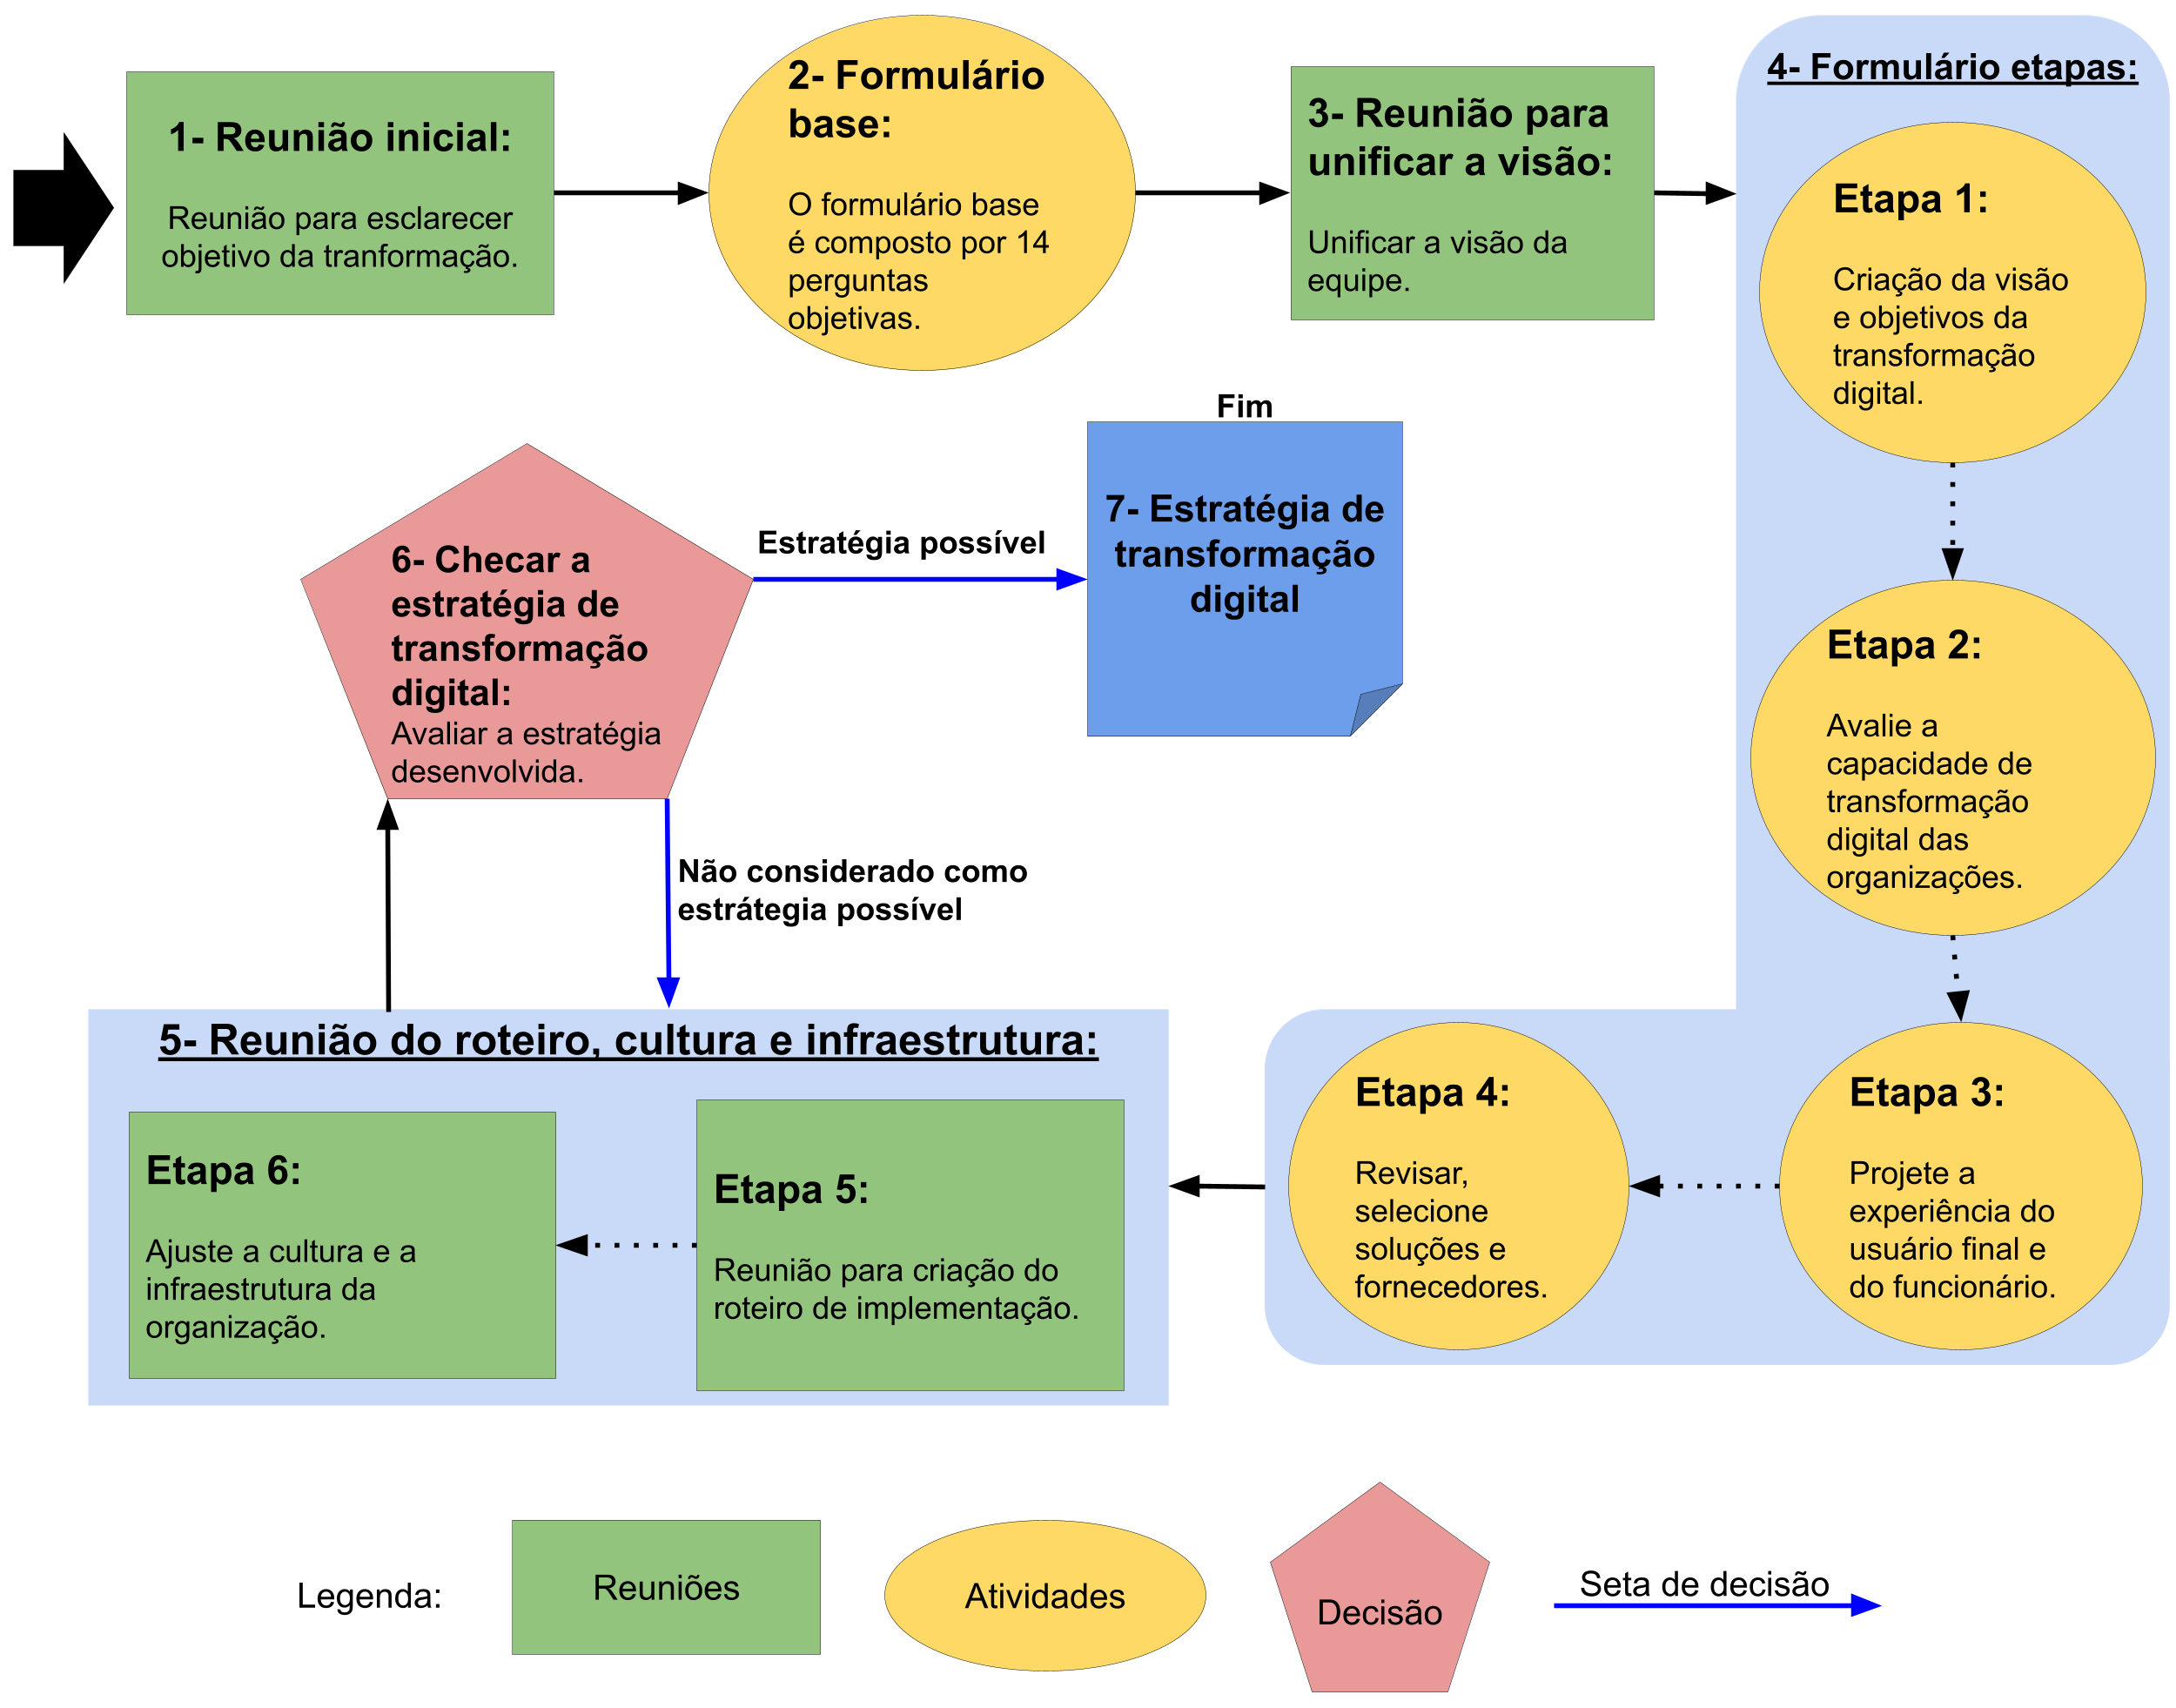
\includegraphics[scale=0.18]{figuras/mapETD.png}
    \caption{Diagrama do processo para elaborar uma estratégia de transformação digital.}
    \label{fig:mapETD}
\end{figure}



\section{Reunião inicial}\label{sec:reuniaoInicial}

O primeiro passo é realizar uma reunião, em que devem participar todas as partes interessadas. A reunião deve abordar minimamente os seguintes itens:

\begin{itemize}
    \item O que é a transformação digital e a sua importância.
    \item Estratégia de transformação digital e a sua importância.
    \item Como devem ocorrer as etapas seguintes e os objetivos.
    \item Esclarecer qualquer outra dúvida que os participantes tenham inicialmente.
\end{itemize}

O objetivo desta etapa é garantir que todos os participantes estejam cientes do processo que se inicia.



\section{Formulário base}\label{sec:atividadeFormBase}

A segunda etapa, tem o objetivo de sumarizar todas as características que devem ser buscadas pela organização, durante a transformação digital. Todos os participantes devem preencher o formulário base de maneira individual.



\section{Reunião para unificar a visão}

A reunião para unificar a visão, tem o objetivo de consolidar em uma única perspectiva, os objetivos da transformação digital definidas de maneira individual na atividade "\nameref{sec:atividadeFormBase}". Assim, partindo de uma única sumarização, todas as próximas atividades, mesmo que diferentes, tendem a chegar em um mesmo objetivo.

Na reunião para unificar a visão, um dos participantes deve ficar responsável por preencher um novo formulário base, através do consenso entre todos os participantes. Para cada pergunta do formulário, todos os participantes devem expor suas respostas, e o(s) participante(s) que não escolheu a resposta da maioria, deve expor o motivo de sua escolha. Se ainda sim, a maioria não concordar, a resposta da maioria deve ser marcado no formulário base.

Ao final da reunião, o formulário base preenchido deve ser disponibilizado para todos os participantes, e está sumarização dos objetivos deve ser considerado para as atividades subsequentes.


\section{Formulário de atividades}\label{sec:formAtividade}

O formulário de atividades é composto por 4 etapas, que devem ser realizadas de maneira individual e descritas com o máximo de detalhes possível. As atividades da etapa englobam objetivos, futuras experiências com clientes e funcionários, aspectos da infraestrutura, capacidade e flexibilidade da organização, maneiras de simplificar o trabalho dos funcionários, facilitar o acesso do cliente, e por fim, deve-se realizar uma seleção de soluções e de fornecedores.

Todas as atividades realizadas pelo "\nameref{sec:formAtividade}" deve ser entregue, ou acessada pelo responsável da estratégia de transformação digital, definido pelo "\nameref{sec:formBase}". Onde o mesmo deve realizar uma compilação dos resultados, e transcrever os objetivos específicos, as capacidades, experiência de clientes e funcionários e potenciais soluções e fornecedores.

\section{Reunião do roteiro, cultura e infraestrutura}\label{sec:reuniaoRoteiroCulturaInfraestrutura}

A compilação dos resultados do "\nameref{sec:formEtapas}" devem ser disponibilizado para todos os participantes antes da "\nameref{sec:reuniaoRoteiroCulturaInfraestrutura}". Duas etapas devem ser realizadas nesta reunião, sendo elas, a criação do roteiro de implementação (Etapa 5), e também a identificação de ajustes na cultura e infraestrutura da organização (Etapa 6). O responsável por elaborar a estrategia deve realizar anotações sobre cada atividade, para que posteriormente complete a documentação contendo a estratégia de transformação digital.\\

A etapa 5 é composta pelas seguintes atividades:
\begin{itemize}
    \item De acordo com as etapas anteriores, descreva o primeiro passo/preparação para a implementação.
    
    \item Descreva os passos da implementação em si.
    
    \item Descreva os passos no âmbito financeiro da implementação.
    
    \item Descreva também o passo final/finalização da implementação.\\
\end{itemize}

E a etapa 6, composta pelas seguintes atividades:
\begin{itemize}
    \item Descreva ajustes da cultura que devem ser construídas ou adaptadas na organização.
    
    \item Descreva modificações que devem ocorrer na infraestrutura da organização.
    
    \item Descreva funções de um equipe dedicada, juntamente com o nome de um possível especialista ou "a contratar", quando a organização não tem um colaborador apto para uma nova função.
    
    \item Para ajustar a cultura e a infraestrutura, recursos financeiros serão necessários?
\end{itemize}



\section{Checagem da estratégia}\label{sec:checagemDaEstrategia}

Esta etapa deve ser realizada pelos idealizadores da organização, que consiga identificar implementações que podem não ser viáveis para a organização, assim como também identificar problemas no plano e se as soluções selecionadas possam, de alguma maneira, não serem disponibilizadas para a organização.


\section{Finalização}

Por fim, um único documento contendo o plano e instruções, que compilados se caracterizam em uma estratégia de transformação digital, deve ser apresentado para toda a organização. Estratégia essa que deve ser iniciada quanto antes, garantindo assim a validade e eficiência do plano elaborado.